\documentclass[12pt,twoside]{article}

\usepackage[english]{babel}
\usepackage[utf8]{inputenc}
\usepackage{sansmathfonts}
\usepackage[T1]{fontenc}
\renewcommand*\familydefault{\sfdefault} %% Only if the base font of the document is to be sans serif
\usepackage{multicol,lipsum}
\usepackage{amsmath,cancel}
\usepackage{amssymb,amsthm,dsfont,mathrsfs}
\usepackage[colorinlistoftodos]{todonotes}
\usepackage{geometry}
\geometry{
a4paper,
total={170mm,257mm},
left=20mm,
top=15mm,
bottom=22mm,
}
\usepackage{natbib}
\usepackage{soul}
\usepackage{setspace}
\usepackage{hyperref}
\usepackage{xcolor}
\usepackage{graphicx}
\usepackage{tikz}
\usepackage{siunitx}
\graphicspath{ {imagens/} }
\usepackage{fancyhdr}
\pagestyle{fancy}
\renewcommand{\headrulewidth}{0pt}

\color{darkgray}
\newcommand{\T}[1]{\vspace{0.4cm}\textbf{\large#1}}
\newcommand{\TW}[1]{\textbf{\large#1}}

\newcommand{\TM}[1]{\vspace{0.2cm} \textbf{#1}}

\newcommand{\M}[1]{
\vspace{-0.6cm}
\begin{flalign*}
#1&
\end{flalign*}
\vspace{-0.6cm}
}


\definecolor{bluebell}{rgb}{0.25, 0.35, 0.89} 
\definecolor{laranja}{rgb}{0.87, 0.48, 0.25} 
\definecolor{verde}{rgb}{0, 0.54, 0.44} 
\definecolor{babypink}{rgb}{1, 0.42, 0.52} 
\definecolor{rosa}{rgb}{1, 0.72, 0.77} 
\definecolor{cinza}{rgb}{0.3, 0.3, 0.3}  
\definecolor{iris}{rgb}{0.25, 0.35, 0.89}  
\definecolor{babyblue}{rgb}{0.13, 0.59, 0.95}

\setlength\columnsep{30pt}

\setlength{\parindent}{0cm}
\setlength{\fboxrule}{1.3pt}  % <-- Aumenta a espessura

\newcommand{\Formula}[1]{
\begin{center}
\color{iris}
\fcolorbox{rosa}{white}{
\(
\begin{array}{c}
#1
\end{array}
\)
}
\color{cinza}
\end{center}
}

\begin{document}
\pagenumbering{gobble}


\includegraphics[width=4cm]{Logo2.png}
\begin{center}
    \textbf{\Huge \textcolor{bluebell}{Função Quadrática}}
\end{center}
\vspace{0.5cm}

\begin{multicols}{2}

% ── DEFINIÇÃO ────────────────────────────────────────────────────────────────
\TW{Definição}

\Formula{f(x) = ax^2 + bx + c \quad (a \neq 0)}

$D(f) = \mathbb{R}$. O gráfico é uma \textbf{parábola}.

\fcolorbox{laranja}{white}{\parbox{0.85\linewidth}{
\small A \emph{equação} $ax^2+bx+c=0$ pergunta quando $f(x)=0$.
A \emph{função} descreve o comportamento completo.
}}

% ── GRÁFICO ───────────────────────────────────────────────────────────────────
\TW{Gráfico — A Parábola}

$a > 0$ → concavidade \textbf{para cima} (mínimo).

$a < 0$ → concavidade \textbf{para baixo} (máximo).

Eixo de simetria: $x_v = \dfrac{-b}{2a}$.

\begin{center}
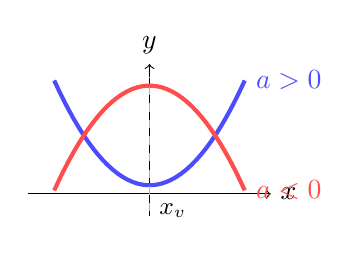
\begin{tikzpicture}[scale=0.55]
  \draw[->] (-2.8,0) -- (2.8,0) node[right] {$x$};
  \draw[->] (0,-0.5) -- (0,3) node[above] {$y$};
  \draw[blue!70, line width=1.5pt, domain=-2.2:2.2, samples=40]
    plot (\x, {0.5*\x*\x + 0.2}) node[right] {$a>0$};
  \draw[red!70, line width=1.5pt, domain=-2.2:2.2, samples=40]
    plot (\x, {-0.5*\x*\x + 2.5}) node[right] {$a<0$};
  \draw[dashed, gray!60] (0,-0.4) -- (0, 2.7);
  \node[below right, font=\small] at (0,0) {$x_v$};
\end{tikzpicture}
\end{center}

% ── VÉRTICE ───────────────────────────────────────────────────────────────────
\TW{Vértice da Parábola}

\Formula{x_v = \dfrac{-b}{2a} \qquad y_v = \dfrac{-\Delta}{4a}}

$y_v$ é o \textbf{mínimo} de $f$ se $a > 0$; \textbf{máximo} se $a < 0$.

\TM{Exemplo — $f(x) = x^2 - 10x + 9$}

\M{
  \Delta &= 100-36 = 64\\
  x_v &= 5 \qquad y_v = \dfrac{-64}{4} = -16
}

Vértice: $V(5,\,-16)$ — mínimo.

% ── ZEROS ─────────────────────────────────────────────────────────────────────
\TW{Zeros da Função}

São os valores $x$ onde $f(x) = 0$ (raízes de Bhaskara).

Forma fatorada ($\Delta \geq 0$):

\Formula{f(x) = a(x-x_1)(x-x_2)}

\TM{Exemplo — $f(x) = 2x^2 - 8x + 6$}

$\Delta = 64-48 = 16$; $x_1 = 1$, $x_2 = 3$.

$f(x) = 2(x-1)(x-3)$ \checkmark

% ── ESTUDO DO SINAL ───────────────────────────────────────────────────────────
\TW{Estudo do Sinal}

Com $\Delta > 0$ e zeros $x_1 < x_2$:

$a > 0$ → $f(x) < 0$ \textbf{entre} $x_1$ e $x_2$; positiva fora.

$a < 0$ → $f(x) > 0$ \textbf{entre} $x_1$ e $x_2$; negativa fora.

Se $\Delta < 0$: $f(x)$ tem sinal constante igual ao de $a$.

% ── DOMÍNIO E IMAGEM ─────────────────────────────────────────────────────────
\TW{Domínio, Imagem e Variação}

$D(f) = \mathbb{R}$

\Formula{\text{Im}(f) = \begin{cases} [y_v, +\infty) & a > 0 \\ (-\infty, y_v] & a < 0 \end{cases}}

$a > 0$: decrescente em $(-\infty, x_v]$, crescente em $[x_v, +\infty)$.

$a < 0$: crescente em $(-\infty, x_v]$, decrescente em $[x_v, +\infty)$.

% ── OTIMIZAÇÃO ───────────────────────────────────────────────────────────────
\TW{Otimização}

\TM{Altura máxima — $h(t) = -5t^2 + 20t$}

\M{t_v = 2\,\text{s} \qquad h_{\max} = 20\,\text{m}}

\TM{Área máxima — cerca de 40 m}

$A(x) = x(20-x) = -x^2 + 20x$

$x_v = 10 \;\Rightarrow\; A_{\max} = 100\,\text{m}^2$

\TM{Lucro máximo — $L(x) = -2x^2 + 80x - 600$}

$x_v = 20$ unidades $\;\Rightarrow\; L_{\max} = \text{R\$}\,200$

\end{multicols}

\lfoot{\scriptsize © Copyright, Pratique Já}
\cfoot{\large \textcolor{bluebell}{pratiqueja.com}}
\end{document}
